\documentclass[letterpaper]{article}
\usepackage[submission]{aaai2027}
\usepackage[hyphens]{url}
\usepackage{graphicx}
\urlstyle{rm}
\def\UrlFont{\rm}
\usepackage{natbib}
\usepackage{caption}
\frenchspacing

\usepackage{amsmath,amssymb}
\usepackage{booktabs}

\pdfinfo{
/TemplateVersion (2027.1)
}

\setcounter{secnumdepth}{2}

\title{Supplementary Material}
\author{Anonymous Submission}
\affiliations{}

\begin{document}
\maketitle

This document reports method details, the complete baseline comparison, case accounting, and secondary analyses under the same fixed subsets, backbones, and unmodified benchmark interfaces as the main paper.
It expands the evidence map by connecting each contrast to the mechanism and inferential unit it measures.
Following the main paper, we abbreviate the three benchmarks as DiagnosisArena (DA), MedCaseReasoning (MCR), and Open-XDDx (OX).
Sections marked \emph{extended analysis} report quantities computed from the persisted per-case records of the same evaluation passes, together with a small number of re-measurements carried out under the same frozen protocol and identified as such where they appear.

\section{Method Details and Audit Rationale}

This section fixes the notation used throughout the main paper and this supplement (Table~\ref{tab:notation}) and then gives, mechanism by mechanism, the implementation detail behind each component the main paper describes at the level of its function.

\begin{table}[tb]
\centering
\small
\begin{tabular}{@{}lp{5.0cm}@{}}
\toprule
Symbol & Meaning \\
\midrule
$\mathcal{K}$ & corpus shared by retrieval-based methods \\
$k_{\mathrm{out}}$ & maximum number of emitted diagnoses \\
$B_t$ & shared belief state at stage $t$ \\
$B_{\mathrm{evid}}$ & maximum selected L1 evidence facts supplied to the updater \\
$N$ & size of the updated-score pool before bounded decoding \\
$r$ / $\sim$ & pairwise semantic predicate / its component closure \\
\bottomrule
\end{tabular}
\caption{Notation used consistently in the main paper and supplement.}
\label{tab:notation}
\end{table}

\paragraph{Case-adaptive organization.}
The Level-1 (L1) partition is constrained to use one case-specific comparison axis, labels broader than a single disease, near-exclusive sibling families, a residual family, and optional low-prior families for cannot-miss alternatives.
It serves as a temporary coordinate system specialized to the current syndrome.
If a high-ranked recalled disease has no suitable parent, one non-reducing gap-fill call may enlarge or add families.
Gap-fill supplies a targeted structural repair for parent absence.

\paragraph{Candidate-relative evidence.}
The deployed anti-prototype selector discounts the most tempting vignette prototype and requires a fact to remain discriminative under comparison with live alternatives; it may abstain.
Each consumed fact updates at most one primary support target and one distinct opposing target among L1 families.
Replacing this selector with a salience selector or removing its discrimination hints changes DA Top-1 by $0.04$ (both $p>0.4$), whereas replacing its case-adaptive input axis sharply reduces fact selection and ranking.
This contrast locates the observed gain in the interaction between the case axis and candidate-relative selection.

\paragraph{Concept-aware compression.}
Synonym crowding causes two distinct failures.
\emph{Slot dilution} pushes competing concepts below the output cutoff; \emph{decision splitting} distributes support across several strings for one concept when the scoring contract expects a canonical name.
Concept-aware compression addresses both by preserving clinical equivalence while reallocating slots to distinct hypotheses.

\paragraph{Equivalence construction.}
The implementation first applies a gold-blind pairwise predicate $r$ to candidate labels at the benchmark's scored granularity.
The predicate is symmetrized, candidates become vertices in an undirected graph, and connected components define the transitive closure $\sim$ used for competition.
Within each component, the highest pre-compression rank is retained as representative; ties preserve the frozen input order.
This is single-linkage closure: two labels may share a component through an intermediate chain even when $r$ does not directly relate the endpoints.
The quotient guarantee applies to the closed relation $\sim$; the pairwise predicate, closure, and representative rule are independently auditable implementation components.

\paragraph{Belief-state transition.}
The persisted state is $B_t=(G_t,q_t,s_t,E_t)$: hierarchy, concept-class assignment, relative leaf scores, and evidence annotations.
Local annotation returns updated leaf fields $B_{t+1}=U(B_t,e_t)$.
The arm without score write-back constructs the global pool from the stale $s_t$ fields; the evidence-conditioned score write-back arm replaces them with the corresponding fields in $s_{t+1}$ before any pool or decoder is run.
These updated scores act as relative ranking quantities rather than calibrated probabilities.

\paragraph{Bounded multi-candidate decoding.}
If family $g$ submits $b_g$ leaves, fixing $b_g{=}1$ makes every local ordering error irreversible and hides the eliminated leaf from global arbitration.
APHHM instead permits $b_g{=}2$ when the local margin is small or evidence is thin, or discards family quotas and decodes from the Top-$N$ updated-score pool; OX uses $N{=}15$ before emitting $k_{\mathrm{out}}{=}5$ names.
The cap sweep scores $0.657$, $0.651$, and $0.649$ for cap${=}1$, cap${=}6$, and cap${=}999$, respectively, making decoding robust across these settings on the current OX subset.
Table~\ref{tab:decoder-contract} states what distinguishes the decoder arms operationally, since they differ in the contract they enforce rather than in the search they perform.

\begin{table}[tb]
\centering
\small
\begin{tabular}{@{}p{2.15cm}p{4.45cm}@{}}
\toprule
Decoder arm & Operation on the same score-updated tree \\
\midrule
Closed panel & Restrict discussion to the Top-$15$ pool and project the five emitted names back into that pool. \\
Updated-score-pool decoder & Decode from the same Top-$15$ pool without the closed-panel discussion step. \\
Direct updated-score Top-5 & Emit the five highest-scored leaves directly, without discussion. \\
\bottomrule
\end{tabular}
\caption{Operational distinction among the OX decoder arms.}
\label{tab:decoder-contract}
\end{table}

\section{Stage-Aware Attribution and Interventions}

A failed case is assigned to the earliest applicable stage, and later stages are examined only once earlier ones succeed.
The main paper lists each stage with the intervention it requires; Table~\ref{tab:stages} adds the failure condition that defines each stage, so that an evaluation-interface error is never reported as insufficient recall.
The attribution measured on DiagnosisArena, together with the counterfactual intervention implied by an unstratified reading, appears in the main paper.

\begin{table*}[t]
\centering
\small
\begin{tabular}{lp{7.4cm}p{4.3cm}}
\toprule
Stage & Failure condition & Appropriate intervention \\
\midrule
Parent absent & No clinically acceptable Level-1 (L1) family can host the target disease. & Revise or repair the case axis. \\
Leaf absent & A suitable family exists, but no equivalent Level-2 (L2) disease leaf is generated. & Improve branch-conditioned recall. \\
Local elimination & The target leaf exists but is removed before global decoding. & Preserve a bounded local frontier. \\
Global misranking & The target reaches the global pool but falls below the cutoff. & Improve state updates or global arbitration. \\
Binding failure & The target ranks sufficiently high, but the scoring interface records no canonical binding. & Standardize name--concept mapping. \\
\bottomrule
\end{tabular}
\caption{Stage-aware attribution separates structural, ranking, and evaluation-interface failures. Each row licenses a different repair, so the assigned stage determines which intervention is warranted.}
\label{tab:stages}
\end{table*}

\section{Full-Cohort Failure Attribution (extended analysis)}
\label{sec:full-cohort}

The stage audit in the main paper covers the cases flagged by one automatic coverage probe.
The persisted per-case records additionally support an attribution over \emph{every} evaluated case on all three benchmarks, which we report here because the two views answer different questions.
Table~\ref{tab:full-cohort} assigns each of the $100$ cases per benchmark to the earliest stage at which the target is lost, using the recorded structural-reachability and local-frontier flags.

\begin{table}[tb]
\centering
\small
\begin{tabular}{@{}lccc@{}}
\toprule
Stage & DA & MCR & OX \\
\midrule
Apparent coverage miss & $20$ & $22$ & $15$ \\
Local elimination & $17$ & $20$ & $\mathbf{40}$ \\
Global misranking & $\mathbf{22}$ & $10$ & $6$ \\
\midrule
Target delivered and scored & $40$ & $46$ & $38$ \\
Unscorable record & $1$ & $2$ & $1$ \\
\bottomrule
\end{tabular}
\caption{Earliest-stage attribution over all evaluated cases ($n{=}100$ per benchmark). Bold marks the dominant failure stage on each benchmark. The apparent-coverage-miss row is the bucket that the main paper's audit resolves further; Table~\ref{tab:coverage-resolved} resolves it on the deployed configuration.}
\label{tab:full-cohort}
\end{table}

\begin{figure*}[t]
\centering
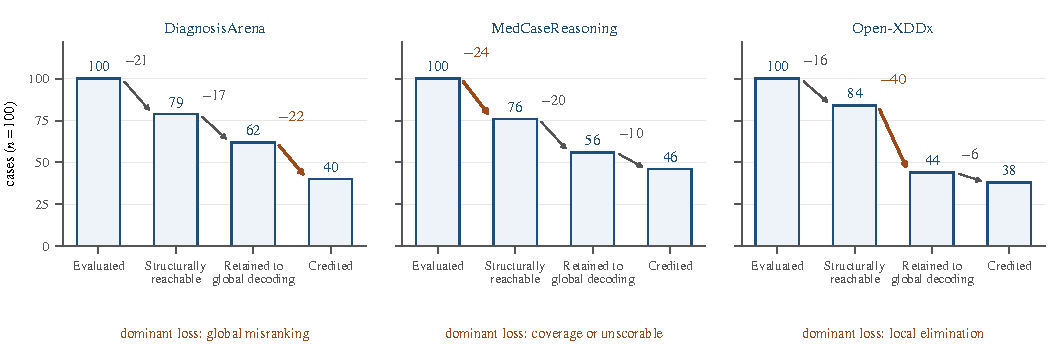
\includegraphics{figures/supp_funnel.pdf}
\caption{The same attribution read as a cumulative funnel. Bars give the cases still carrying the target at each stage and arrows the loss at each transition, with the dominant loss of each benchmark in the second colour. The first transition merges the apparent-coverage-miss row with the one or two unscorable records, so the bar heights coincide with the reachable, frontier and scored columns of Table~\ref{tab:utilisation}. The three benchmarks lose their targets at three different stages: predominantly at global misranking on DiagnosisArena, at the coverage bucket on MedCaseReasoning, and at local elimination on Open-XDDx.}
\label{fig:funnel}
\end{figure*}

Two observations follow.
First, the intermediate stages are not empty over the full cohort: local elimination and global misranking together account for $39$ of the $60$ DiagnosisArena failures, $30$ of $54$ on MedCaseReasoning, and $46$ of $62$ on Open-XDDx.
The audit in the main paper conditions on an apparent coverage gap and therefore reports zero cases at these stages by construction; it should not be read as evidence that local and global stages do not fail.
Second, the dominant stage differs across benchmarks: local elimination on Open-XDDx, global misranking on DiagnosisArena, and the apparent coverage bucket on MedCaseReasoning (Figure~\ref{fig:funnel}).
Each mechanism examined in the main paper was evaluated on the benchmark where its target failure mode is dominant, which is a property of the evidence design rather than a result.
It also yields a prediction for cross-benchmark replication: evidence-conditioned score write-back, which acts on the local-to-global transition, should transfer with a larger margin to benchmarks whose failures concentrate at local elimination than to those dominated by global misranking.

\paragraph{Resolving the apparent coverage bucket on the deployed configuration.}
Both the main paper's audit and Table~\ref{tab:full-cohort} count twenty apparent coverage misses on DiagnosisArena, but the two buckets are selected by different probes: the audit uses a family-level coverage probe, whereas Table~\ref{tab:full-cohort} uses a leaf-level probe on the configuration whose scores the main paper reports.
The two sets of twenty intersect in eight cases, so what follows is a second and largely disjoint sample of the same phenomenon rather than a restatement of the audited split.
We resolve it by re-applying the same lexical leaf predicate to the deployed configuration's own records, with the target name as the matching text.

\begin{table}[tb]
\centering
\small
\begin{tabular}{@{}p{4.55cm}cc@{}}
\toprule
Resolution & Cases & Interface bound \\
\midrule
Binding failure: an equivalent leaf is on the tree and no binding is recorded & $7$ & no \\
Probe conflict: an equivalent leaf is on the tree and a binding is recorded & $7$ & yes \\
Structural absence: no lexically equivalent leaf & $6$ & --- \\
\bottomrule
\end{tabular}
\caption{The $20$ apparent coverage misses on DA resolved from the deployed configuration's own records. Fourteen of $20$ have an equivalent leaf on the tree, so the apparent gap is predominantly not a generation gap. Separating parent absence from leaf absence within the remaining six requires clinical adjudication of family acceptability and is left to the human audit.}
\label{tab:coverage-resolved}
\end{table}

Fourteen of the $20$ cases carry a lexically equivalent leaf on the tree.
Two probes that share only eight of twenty cases, applied to two configurations and adjudicated by two different predicates, therefore reach the same conclusion: an apparent coverage miss is predominantly not a generation gap.
What changes with the probe is the size of that majority, $18/20$ in the audited subset and $14/20$ here, and not its direction.
The \emph{probe conflict} category is itself informative: in seven cases the internal coverage probe reports the target as absent although the scoring interface records a binding, so automatic coverage counts and interface outcomes disagree on the same case.
This dissociation is the quantitative form of the argument that coverage statistics should not be read as recall evidence without a stage assignment.

\section{Stage Hazards and Counterfactual Repair Value (extended analysis)}
\label{sec:hazards}

The attribution in Section~\ref{sec:full-cohort} assigns each case to the earliest stage at which the target is lost, which identifies where failures originate but not how demanding each transition is for the cases that actually reach it.
Reading the same persisted records as a survival process supplies the complementary view.
For each ordered transition Table~\ref{tab:hazards} reports the number of cases still carrying the target when the transition begins, the number lost at it, and the conditional loss rate with a Wilson interval.
Because the funnel is reconstructed from structural records rather than from the scoring judge, the target is matched by the lexical predicate used elsewhere in this supplement, so the terminal rate of the funnel is a lexical credit rate and not the judged accuracy reported in the main paper; the two are different quantities and should not be compared directly.

\begin{table*}[t]
\centering
\small
\begin{tabular}{@{}lccc@{\hspace{1.4em}}ccc@{}}
\toprule
 & \multicolumn{3}{c}{MedCaseReasoning} & \multicolumn{3}{c}{Open-XDDx} \\
\cmidrule(lr){2-4}\cmidrule(lr){5-7}
Transition & At risk & Lost & Loss rate [$95\%$ CI] & At risk & Lost & Loss rate [$95\%$ CI] \\
\midrule
Entry $\rightarrow$ family admission & $100$ & $30$ & $0.300$ $[0.219,0.396]$ & $100$ & $1$ & $0.010$ $[0.002,0.054]$ \\
Family $\rightarrow$ leaf generated & $70$ & $1$ & $0.014$ $[0.003,0.077]$ & $99$ & $1$ & $0.010$ $[0.002,0.055]$ \\
Leaf $\rightarrow$ survives family cap & $69$ & $0$ & $0.000$ $[0.000,0.053]$ & $98$ & $0$ & $0.000$ $[0.000,0.038]$ \\
Cap $\rightarrow$ arbitration pool & $69$ & $17$ & $0.246$ $[0.160,0.360]$ & $98$ & $5$ & $0.051$ $[0.022,0.114]$ \\
Arbitration $\rightarrow$ routed ranking & $52$ & $1$ & $0.019$ $[0.003,0.101]$ & $93$ & $0$ & $0.000$ $[0.000,0.040]$ \\
Routing $\rightarrow$ emitted list & $51$ & $0$ & $0.000$ $[0.000,0.070]$ & $93$ & $1$ & $0.011$ $[0.002,0.058]$ \\
Emitted $\rightarrow$ lexical credit & $51$ & $9$ & $0.176$ $[0.096,0.303]$ & $92$ & $0$ & $0.000$ $[0.000,0.040]$ \\
\midrule
Terminal lexical credit rate & \multicolumn{3}{c}{$0.42$} & \multicolumn{3}{c}{$0.92$} \\
\bottomrule
\end{tabular}
\caption{Conditional loss rate at each ordered transition, with Wilson intervals, over the $100$ evaluated cases per benchmark. \emph{At risk} counts the cases still carrying the target when the transition begins. The terminal figure is a lexical credit rate computed from the persisted structural records: on MedCaseReasoning it credits the single target, and on Open-XDDx it credits a case in which at least one target of the differential is matched. Neither is the judged endpoint reported in the main paper.}
\label{tab:hazards}
\end{table*}

The funnel has the same shape on both benchmarks at very different absolute levels.
The transitions governed by deterministic bookkeeping---the per-family cap, the routing of the arbitrated ranking, and the projection into the emitted list---lose almost nothing, and their upper confidence limits remain within a few percentage points even where no loss is observed at all.
The losses concentrate at the two transitions that involve a model decision, admission into a Level-1 family and global arbitration, and on MedCaseReasoning also at the final transition from the emitted list to a recorded credit, which is the evaluation-interface stage examined in Section~\ref{sec:ial}.

The same records bound what repairing a single stage could return.
For each transition we ask what the terminal rate would become if every case lost there were carried forward and thereafter behaved like the cases that already survive it.
This is an upper bound rather than an estimate, because it grants the repaired cases the favourable conditional credit rate of the survivors; it is reported only to rank the stages against one another.
On MedCaseReasoning the bound is $+0.180$ for family admission and $+0.137$ for arbitration, against no more than $+0.009$ for any deterministic transition, with the interface transition at $+0.090$.
On Open-XDDx, where the funnel is shallow throughout, the largest bound is $+0.049$ at arbitration and every other transition is at most $+0.010$.

Two consequences follow for how the remaining error should be read.
The bookkeeping stages are not where headroom lies: an oracle that never lost a case at the cap, at routing, or at projection would move the terminal rate by at most one percentage point on either benchmark, which is the quantitative form of the design intention that these stages act as lossless carriers rather than as filters.
The stages that do carry headroom are the two substantive decisions the main paper already isolates, construction of the case axis and global arbitration, together with the evaluation interface, which on MedCaseReasoning is comparable in size to arbitration itself and is not a property of the reasoning system at all.

\section{Recall Utilisation (extended analysis)}
\label{sec:utilisation}

The main paper frames difficult diagnosis as a tension between coverage and discrimination but reports only end-task scores.
Table~\ref{tab:utilisation} makes the intermediate quantities explicit for the full model.

\begin{table}[tb]
\centering
\small
\begin{tabular}{@{}lcccc@{}}
\toprule
Benchmark & Reachable & Frontier & Scored & Utilisation \\
\midrule
DA & $79$ & $62$ & $40$ & $0.506$ \\
MCR & $76$ & $56$ & $46$ & $0.605$ \\
OX & $84$ & $44$ & $38$ & $0.452$ \\
\bottomrule
\end{tabular}
\caption{Recall utilisation of the full model. ``Reachable'' counts cases whose target is structurally present, ``frontier'' those retained into global decoding, and ``scored'' those credited by the benchmark. Utilisation is scored divided by reachable. Open-XDDx uses the single proxy target of the cascade harness rather than the full multi-label set, so its row is a within-cascade quantity and is not comparable to the reported micro-F1.}
\label{tab:utilisation}
\end{table}

Between $45\%$ and $61\%$ of structurally available targets reach the score, so roughly half of the coverage the system already holds is lost at later stages; the three columns of this table are the last three bars of each panel of Figure~\ref{fig:funnel}.
Flat pipelines do not persist an intermediate candidate ledger, so this quantity cannot be computed for them under the same definition; the ability to state it is a property of the staged representation rather than a comparison.

\section{Evaluation Protocol Details}

Each evaluation uses the first 100 cases under a fixed benchmark order; the released artifacts include the corresponding subset manifests.
All retrieval arms share the same indices and \path{meta-llama/llama-3.3-70b-instruct} backbone~\cite{llama33}; MCR reasoning recall uses the \texttt{gemini-2.5-flash} endpoint~\cite{gemini25flash} with a fixed prompt and no lexical substitution.
Each point estimate is one fixed evaluation pass per configuration.
Candidate enumeration uses temperature zero, although provider-side nondeterminism may remain; paired resampling is used for uncertainty rather than for averaging repeated system runs.
Gold labels are excluded from generation, evidence selection, state update, and arbitration, and every reported result uses the original benchmark scoring interface.
Table~\ref{tab:case-accounting} reconciles the raw, scored, and audited case counts on each benchmark.

\begin{table}[tb]
\centering
\small
\begin{tabular}{@{}lrrr@{}}
\toprule
Dataset & Raw & Main scored & Audit $n$ \\
\midrule
DA & 100 & 100 & 20 \\
MCR & 100 & 98 & 42 \\
OX & 100 & 100 & 100 \\
\bottomrule
\end{tabular}
\caption{Case accounting. Audit $n$ denotes the stage audit on DA, perturbable-partition audit on MCR, and state factorial on OX. Two MCR cases lack a common fixed-judge score; endpoint tables state further conditioning explicitly.}
\label{tab:case-accounting}
\end{table}

\section{Complete Baseline Table}

The result table in the main paper is restricted to the arms that share one backbone, which is the condition under which the reported differences are attributable to method rather than to model capacity.
Table~\ref{tab:all-baselines} reproduces it in full and restores the one completed arm held out of it.
DiagnosisGPT-6B runs on its own $6$B backbone and so cannot be placed on the controlled axis; it is reported here as a local-backbone reference point rather than as a baseline under the shared-backbone protocol, and no claim in either document rests on the comparison against it.
Every other entry is identical to the corresponding main-paper value, so the two tables can be read interchangeably outside that row.

\begin{table*}[t]
\centering
\small
\begin{tabular}{@{}lcccccc@{}}
\toprule
& \multicolumn{3}{c}{DA} & \multicolumn{2}{c}{MCR} & OX \\
Method & @1 & @2 & MRR@2 & Acc@1 & R-Recall & micro-F1 \\
\midrule
\textbf{APHHM} & \textbf{0.71} & \textbf{0.78} & \textbf{0.748} & \textbf{0.50} & \textbf{0.753} & \textbf{0.651} \\
MEDDxAgent & 0.62 & 0.71 & 0.665 & 0.24 & 0.412 & 0.491 \\
MAC & 0.61 & 0.67 & 0.640 & 0.23 & 0.527 & 0.570 \\
Dual-Inf & 0.60 & 0.70 & 0.650 & 0.17 & 0.444 & 0.507 \\
i-MedRAG & 0.60 & 0.67 & 0.635 & 0.19 & 0.482 & 0.419 \\
MDAgents & 0.58 & 0.67 & 0.625 & 0.20 & 0.570 & 0.543 \\
Self-refine & 0.57 & 0.62 & 0.595 & 0.21 & 0.447 & 0.530 \\
Flat rerank & 0.56 & 0.63 & 0.595 & 0.17 & 0.404 & 0.495 \\
CoT+RAG & 0.55 & 0.63 & 0.590 & 0.22 & 0.478 & 0.466 \\
Direct CoT & 0.54 & 0.61 & 0.575 & 0.18 & 0.510 & 0.543 \\
Chain-of-Diagnosis + shared corpus & 0.54 & 0.55 & 0.545 & 0.14 & 0.430 & 0.475 \\
Self-consistent CoT (5 samples) & 0.52 & 0.61 & 0.565 & 0.19 & 0.369 & 0.539 \\
Flat beam search & 0.52 & 0.60 & 0.560 & 0.21 & 0.447 & 0.510 \\
Medprompt-style & 0.52 & 0.57 & 0.545 & 0.18 & 0.294 & 0.522 \\
MedRAG & 0.48 & 0.52 & 0.500 & 0.17 & 0.557 & 0.485 \\
DiagnosisGPT-6B$^{\dagger}$ & 0.14 & 0.14 & 0.140 & --- & --- & --- \\
\midrule
Flat rerank $\times 10$ (RRF) & 0.47 & 0.59 & 0.530 & 0.15 & 0.383 & 0.487 \\
\bottomrule
\end{tabular}
\caption{Every completed baseline arm under the unmodified benchmark interfaces. $^{\dagger}$DiagnosisGPT-6B is shown as a local-backbone reference point.}
\label{tab:all-baselines}
\end{table*}

\section{Call-Count Audit}

The approximately nine-call structural proxy reproduces a tree-derived schedule and provides an intermediate inference-volume point.
The ten-trajectory flat reranking control, denoted Flat rerank $\times 10$ (RRF), fuses ten independently generated retrieve--rerank lists with reciprocal rank fusion.
The resource axis is mean model calls per case, measured from LLM cache entries.

\begin{table}[tb]
\centering
\small
\begin{tabular}{@{}lccccc@{}}
\toprule
Dataset & APHHM & Native & Proxy & Flat $\times 10$ & Ratio \\
\midrule
DA & 94.3 & 2.0 & 9.24 & 92.4 & 0.98 \\
OX & 68.6 & 2.0 & 8.98 & 89.8 & 1.31 \\
MCR & 81.2 & 2.0 & 9.32 & 93.2 & 1.15 \\
\bottomrule
\end{tabular}
\caption{Mean model calls per case ($n{=}100$). Flat rerank $\times 10$ (RRF) is matched within $2\%$ on DA and is call-richer than APHHM on OX and MCR.}
\label{tab:compute-audit}
\end{table}

The ten-trajectory control supplies $0.98\times$, $1.31\times$, and $1.15\times$ the APHHM call count on DA, OX, and MCR, respectively.
The nine-call proxy anchors the lower end of the inference-volume ladder, while the ten-trajectory arm provides the similar-call-count comparison.
Figure~\ref{fig:budget} places the full model on that ladder.
Raising flat inference volume from about two calls per case to about ninety does not improve any of the three end tasks, and the full model sits well above the flat pipeline at a comparable call count on all three, which is the form the resource argument takes once the ladder and the audited call counts are read together.

\begin{figure}[tb]
\centering
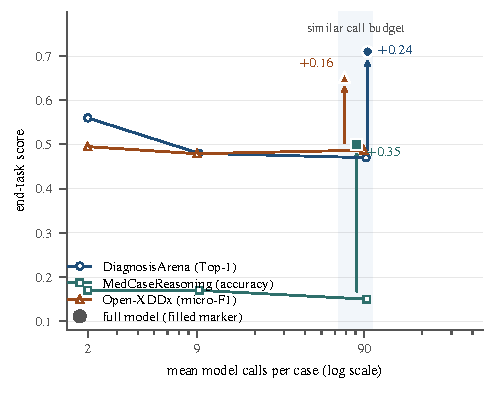
\includegraphics{figures/supp_budget_ladder.pdf}
\caption{End-task score against mean model calls per case on a logarithmic axis. Open markers trace the flat retrieve--rerank pipeline along the inference-volume ladder reported in the main paper, at approximately two, nine and ninety calls per case; filled markers give the full model at the call counts audited in Table~\ref{tab:compute-audit}. A forty-five-fold increase in flat inference volume lowers the score on all three benchmarks, by $0.09$, $0.02$ and $0.008$ respectively, whereas the full model is between $0.16$ and $0.35$ above the ten-trajectory flat control at a comparable budget. Each benchmark uses its own endpoint, so the vertical axis compares configurations within a series and not across series.}
\label{fig:budget}
\end{figure}

\paragraph{Output tokens and latency (extended analysis).}
Because a call-count match need not imply a match in generated volume, we reconstruct the second and third resource axes for the similar-call-count comparison.
Neither arm records an official token ledger, so completion tokens are recounted from the persisted response payloads of both arms with one tokenizer, and per-case latency is read from the persisted timing fields.
The reconstruction is auditable through a fidelity check: the recovered payload count per case is $95.3$ against $94.3$ audited calls on DA and $88.1$ against $81.2$ on MCR, so the two are comparable within $1\%$ and $9\%$ respectively.
The Open-XDDx records of the full model contain several re-annotation passes, recovering $140.0$ payloads per case against $68.6$ audited calls, so that benchmark admits no comparable reconstruction and is omitted from Table~\ref{tab:resource-axes}.

\begin{table}[tb]
\centering
\small
\begin{tabular}{@{}llccc@{}}
\toprule
Benchmark & Arm & Calls & Output tokens & Latency (s) \\
\midrule
DA & APHHM & $94.3$ & $24{,}781$ & $288.3$ \\
DA & Flat $\times 10$ & $92.4$ & $19{,}414$ & $167.5$ \\
DA & ratio & $1.02$ & $1.28$ & $1.72$ \\
\midrule
MCR & APHHM & $81.2$ & $20{,}496$ & $246.0$ \\
MCR & Flat $\times 10$ & $93.2$ & $17{,}934$ & $177.6$ \\
MCR & ratio & $0.87$ & $1.14$ & $1.39$ \\
\bottomrule
\end{tabular}
\caption{Three resource axes per case for APHHM and the ten-trajectory flat control, Flat rerank $\times 10$ (RRF). Output tokens are reconstructed with one tokenizer from the persisted payloads of both arms and are estimates rather than a billed ledger; input tokens are not recoverable for either arm. Latency reflects one execution environment with differing concurrency and is not a controlled measurement.}
\label{tab:resource-axes}
\end{table}

On the two benchmarks that admit reconstruction, the similar-call-count control generates within a factor of $1.14$--$1.28$ of the full model's completion tokens, so the reported margins are not explained by an order-of-magnitude difference in generated volume on this axis.
Wall-clock latency is $1.4$--$1.7\times$ higher for the staged system, which reflects its sequential stage structure; because the two arms ran under different concurrency settings, we report this axis descriptively and do not treat it as a controlled comparison.

\section{Interpretation Quality on Open-XDDx (extended analysis)}
\label{sec:interp}

Open-XDDx scores an interpretation-accuracy endpoint alongside diagnostic micro-F1.
The main paper reports only micro-F1, and Table~\ref{tab:interp} gives both endpoints here for every arm.

\begin{table}[tb]
\centering
\footnotesize
\begin{tabular}{@{}lcc@{}}
\toprule
Method & micro-F1 & Interpretation \\
\midrule
\textbf{APHHM} & $\mathbf{0.651}$ & $0.354$ \\
MAC & $0.570$ & $0.221$ \\
Direct CoT & $0.543$ & $0.233$ \\
MDAgents & $0.543$ & $0.424$ \\
Self-consistent CoT & $0.539$ & $0.000$ \\
Self-refine & $0.530$ & $0.206$ \\
Medprompt-style & $0.522$ & $0.000$ \\
Flat beam search & $0.510$ & $\mathbf{0.642}$ \\
Dual-Inf & $0.507$ & $0.320$ \\
Flat rerank & $0.495$ & $0.419$ \\
MEDDxAgent & $0.491$ & $0.403$ \\
MedRAG & $0.485$ & $0.224$ \\
Chain-of-Diagnosis & $0.475$ & $0.215$ \\
CoT+RAG & $0.467$ & $0.240$ \\
i-MedRAG & $0.418$ & $0.237$ \\
\bottomrule
\end{tabular}
\caption{Both Open-XDDx endpoints under the unmodified interface, ordered by micro-F1. Chain-of-Diagnosis uses the shared corpus and self-consistent CoT draws five samples. APHHM ranks first on the diagnostic endpoint and fifth on the interpretation endpoint.}
\label{tab:interp}
\end{table}

The two endpoints are close to independent across arms.
Arm-level micro-F1 and arm-level interpretation accuracy correlate at $0.019$ (Pearson) and $-0.036$ (Spearman) over the fifteen arms, and at $-0.105$ and $-0.152$ over the fourteen baselines alone.
The interpretation column is therefore not a refinement of the diagnostic ranking: a position on one endpoint carries almost no information about the position on the other, and the two should be read as separate measurements rather than as a coarse and a fine version of the same one.
Part of that independence is a property of the endpoint rather than of the systems.
Two arms score exactly zero, because an arm that emits a fused ranked list without a per-diagnosis rationale field receives no credit for the diagnoses it names; the column thus responds to output form as well as to explanation content.
Against this background, four arms exceed APHHM on the interpretation endpoint while scoring lower on micro-F1.
APHHM emits its five names by projecting a bounded pool back into a closed panel, which preserves the ranked concepts but compresses the per-diagnosis narrative, and its interpretation score should be read in that light.
We report the endpoint rather than omitting it, and we claim no interpretation-quality advantage.
Separating format sensitivity from explanation quality requires re-rendering rationales for a fixed emitted list under one output contract, which we did not run.
The same near-independence holds between the two MedCaseReasoning endpoints (Section~\ref{sec:decoupling}), so on both benchmarks that score a second endpoint, that endpoint measures something the diagnostic endpoint does not order.

\section{Interface-Attributable Loss (extended analysis)}
\label{sec:ial}

The main paper notes that an offline name-matching pass moves accuracy for several systems.
Table~\ref{tab:ial} states this as a per-system quantity: the interface-attributable loss is the Top-1 gain obtained when the same emitted lists are re-bound with a synonym and bridge repair, with generation and ranking untouched.

\begin{table}[tb]
\centering
\footnotesize
\setlength{\tabcolsep}{3pt}
\begin{tabular}{@{}lcccc@{}}
\toprule
Method & Native & Bound & Loss & $n_{\mathrm{rep}}$ \\
\midrule
Self-refine & $0.57$ & $0.65$ & $0.080$ & $26$ \\
Self-consistent CoT & $0.52$ & $0.58$ & $0.060$ & $20$ \\
Direct CoT & $0.54$ & $0.59$ & $0.050$ & $21$ \\
MEDDxAgent & $0.62$ & $0.67$ & $0.050$ & $17$ \\
Medprompt-style & $0.52$ & $0.57$ & $0.050$ & $16$ \\
MedRAG & $0.48$ & $0.53$ & $0.050$ & $12$ \\
CoT+RAG & $0.55$ & $0.59$ & $0.040$ & $18$ \\
Flat rerank & $0.56$ & $0.60$ & $0.040$ & $12$ \\
MDAgents & $0.58$ & $0.62$ & $0.040$ & $21$ \\
Chain-of-Diagnosis & $0.54$ & $0.58$ & $0.040$ & $14$ \\
Flat beam search & $0.52$ & $0.55$ & $0.030$ & $11$ \\
MAC & $0.61$ & $0.64$ & $0.030$ & $22$ \\
i-MedRAG & $0.60$ & $0.63$ & $0.030$ & $17$ \\
Dual-Inf & $0.60$ & $0.62$ & $0.020$ & $12$ \\
Flat rerank $\times 10$ (RRF) & $0.47$ & $0.49$ & $0.020$ & $14$ \\
\textbf{APHHM} & $\mathbf{0.71}$ & $0.73$ & $\mathbf{0.020}$ & $28$ \\
\bottomrule
\end{tabular}
\caption{Interface-attributable loss on DA Top-1. Chain-of-Diagnosis uses the shared corpus and self-consistent CoT draws five samples. ``Native'' is the reported score under the unmodified interface, ``bound'' applies the offline repair to the same emitted lists, and $n_{\mathrm{rep}}$ counts options whose binding changed. The locally backboned reference arm is omitted because the repair moves no case for it.}
\label{tab:ial}
\end{table}

Every retrieval or agent arm loses accuracy to the binding stage, with a mean of $0.041$ and a range of $0.020$ to $0.080$; the repair reorders eight of the eighteen arms relative to their native ranking.
A reported Top-1 score on this benchmark therefore mixes hypothesis quality with name-normalisation coverage, and system rankings are not invariant to the binding contract.
APHHM carries the smallest loss among arms that the repair moves at all, despite the repair touching the largest number of its options: it emits more options that are already bindable, and the options it does gain were bound to a competing member of the same concept class rather than left empty.
This is consistent with concept-level competition promoting a canonical representative, and it is the endpoint on which the representation choice and the scoring contract interact.
We report all main-paper results under the native interface and use this table only to size the interface effect.

\section{Diagnostic Accuracy and Reasoning Recall (extended analysis)}
\label{sec:decoupling}

MedCaseReasoning scores a diagnostic endpoint and a reasoning-fact recall endpoint from the same trajectory.
Across the fourteen baseline arms these endpoints are nearly independent: the Pearson correlation between arm-level accuracy and arm-level reasoning recall is $0.141$ and the Spearman correlation is $0.190$.
The arm with the highest reasoning recall among baselines scores $0.20$ accuracy, and the arm with the highest accuracy ranks tenth of fourteen on reasoning recall (Table~\ref{tab:decoupling}).

\begin{table}[tb]
\centering
\footnotesize
\setlength{\tabcolsep}{3pt}
\begin{tabular}{@{}lcccc@{}}
\toprule
Method & Acc & R-Recall & on hits & on misses \\
\midrule
MEDDxAgent & $0.24$ & $0.412$ & $0.336$ & $0.436$ \\
MAC & $0.23$ & $0.527$ & $0.525$ & $0.528$ \\
CoT+RAG & $0.22$ & $0.478$ & $0.383$ & $0.505$ \\
Flat beam search & $0.21$ & $0.447$ & $0.533$ & $0.424$ \\
Self-refine & $0.21$ & $0.447$ & $0.545$ & $0.421$ \\
MDAgents & $0.20$ & $0.570$ & $0.573$ & $0.569$ \\
Self-consistent CoT & $0.19$ & $0.369$ & $0.423$ & $0.356$ \\
i-MedRAG & $0.19$ & $0.482$ & $0.599$ & $0.455$ \\
Direct CoT & $0.18$ & $0.510$ & $0.484$ & $0.516$ \\
Medprompt-style & $0.18$ & $0.294$ & $0.213$ & $0.312$ \\
Flat rerank & $0.17$ & $0.404$ & $0.440$ & $0.397$ \\
Dual-Inf & $0.17$ & $0.444$ & $0.442$ & $0.445$ \\
MedRAG & $0.17$ & $0.557$ & $0.546$ & $0.559$ \\
Chain-of-Diagnosis & $0.14$ & $0.430$ & $0.287$ & $0.454$ \\
\bottomrule
\end{tabular}
\caption{Per-case MCR endpoints aggregated by arm, with reasoning recall split by whether the diagnostic endpoint was credited. Chain-of-Diagnosis uses the shared corpus and self-consistent CoT draws five samples. Recall on hits exceeds recall on misses for six of fourteen arms, so a trajectory that recovers more case facts is not systematically the one that names the target.}
\label{tab:decoupling}
\end{table}

Because the two endpoints are close to independent across systems, leading on both is not redundant evidence, and the reasoning-recall margin reported in the main paper is not a restatement of the accuracy margin.

\paragraph{Replication under a second judge (extended analysis).}
The reasoning-recall endpoint is produced by a single judge model, so its absolute level could in principle be a property of that judge rather than of the trajectories it reads.
We therefore re-scored the same persisted trajectories with a second judge model from an unrelated developer (\texttt{deepseek-v4-flash}) under the same prompt and the same fixed contract, changing nothing but the scoring endpoint.
Every arm was re-scored, not only the full model, so the change of judge can be evaluated as a change of ranking rather than as a change of one number.
Table~\ref{tab:second-judge} reports both judges for all fourteen arms that admit the comparison.

\begin{table}[tb]
\centering
\footnotesize
\setlength{\tabcolsep}{3pt}
\begin{tabular}{@{}lccc@{}}
\toprule
Mean reasoning recall & Primary & Second & $\Delta$ \\
\midrule
\textbf{APHHM} & $\mathbf{0.753}$ & $\mathbf{0.495}$ & --- \\
MDAgents & $0.570$ & $0.407$ & $+0.089$ \\
MedRAG & $0.557$ & $0.332$ & $+0.163$ \\
MAC & $0.527$ & $0.327$ & $+0.169$ \\
Direct CoT & $0.510$ & $0.350$ & $+0.146$ \\
i-MedRAG & $0.482$ & $0.310$ & $+0.185$ \\
CoT+RAG & $0.478$ & $0.290$ & $+0.205$ \\
Flat beam search & $0.447$ & $0.313$ & $+0.183$ \\
Self-refine & $0.447$ & $0.279$ & $+0.217$ \\
Dual-Inf & $0.444$ & $0.280$ & $+0.216$ \\
Chain-of-Diagnosis & $0.430$ & $0.220$ & $+0.276$ \\
Flat rerank & $0.404$ & $0.257$ & $+0.238$ \\
Self-consistent CoT & $0.369$ & $0.013$ & $+0.483$ \\
Medprompt-style & $0.294$ & $0.026$ & $+0.470$ \\
\midrule
\multicolumn{4}{@{}l}{\emph{Agreement between the two judges}} \\
Arm-level Spearman / Kendall & \multicolumn{3}{c}{$0.960$ / $0.846$} \\
Per-case Spearman / Pearson & \multicolumn{3}{c}{$0.404$ / $0.421$} \\
Per-case shift & \multicolumn{3}{c}{$-0.258$ (SD $0.327$)} \\
\bottomrule
\end{tabular}
\caption{The MedCaseReasoning reasoning-recall endpoint under the primary judge and under a second judge from an unrelated developer, with the same persisted trajectories, the same prompt, and the same fixed contract. Means are over $100$ cases per arm and $\Delta$ is the paired margin of the full model over that arm under the second judge. Rows are ordered by the primary judge. One further arm is held out; see the text.}
\label{tab:second-judge}
\end{table}

The second judge is markedly more conservative: every arm loses between $0.134$ and $0.356$ of mean recall, and the full model falls from $0.753$ to $0.495$.
Absolute levels from the two judges are therefore not interchangeable, and no claim should rest on the level reported by either.
What the change of judge leaves intact is the comparison itself.
The two judges rank the arms almost identically, at a Spearman correlation of $0.960$ over the fourteen arms and $0.951$ over the thirteen baselines alone; the full model is first under both; and all thirteen paired margins remain positive and remain significant after Holm correction within the family.
The narrowest margin, over the strongest baseline on this endpoint, falls from $+0.183$ $[+0.116,+0.250]$ to $+0.089$ $[+0.025,+0.153]$ and stays clear of zero.
The ordering survives a change of judge while the calibration does not, which is the pattern expected when an endpoint separates trajectories reliably and two judges disagree about how much evidence is required to credit a recalled fact.

Two arms behave differently from the rest and are informative rather than anomalous.
Self-consistent CoT and Medprompt-style fall to $0.013$ and $0.026$, because the trajectories they persist consist of ranked diagnosis names with no accompanying rationale; the second judge credits nothing against them, whereas the primary judge credits between a quarter and a third of the reference reasoning points from the names alone.
These are the same two arms that score exactly zero on the Open-XDDx interpretation endpoint (Section~\ref{sec:interp}), and for the same structural reason, so a single property of those systems is visible on two benchmarks under three different scoring endpoints.
The direction of this effect is worth stating plainly: it means the primary judge is generous to arms that emit no reasoning at all, and therefore that the reasoning-recall margins reported in the main paper are conservative rather than inflated.
It also qualifies the near-independence of the two MedCaseReasoning endpoints reported above, part of which is contributed by arms that have no reasoning content for the recall endpoint to measure.

One arm is excluded from Table~\ref{tab:second-judge}.
The evaluation projection built for MEDDxAgent records its diagnosis names but not its per-diagnosis explanations, which the arm does produce, so both judges read a trajectory with no reasoning content for that arm and neither score is a measurement of the system.
Because the defect is in our extraction rather than in the arm, we hold it out of this comparison instead of reporting a margin against it.
The moderate per-case correlation bounds how much weight the endpoint can carry on its own: it supports the direction and the ordering of the reported margins rather than their magnitude, and validation against human scoring remains outstanding.

\section{Interface Failures: Three Cases (extended analysis)}
\label{sec:cases}

The following three cases come from the apparent-coverage bucket of the deployed DA configuration and illustrate three distinct interface pathologies.
Each was verified against the persisted tree, the emitted ranking, and the recorded option binding; all three received no credit under the unmodified interface.

\paragraph{A canonical name that differs only in capitalisation.}
The benchmark option is \emph{Keloidal scleroderma} and the tree carries a leaf labelled \emph{Keloidal Scleroderma}.
The two strings are identical after case folding.
The interface recorded the relation between option and leaf as unrelated with low confidence and bound no leaf, so a delivered target was scored as absent.

\paragraph{A canonical name that differs only in one punctuation character.}
The benchmark option and the emitted leaf both read \emph{Inflammation-induced ocular neuropathy associated with SARS-CoV-2 induced panuveitis}, and they differ at exactly one position: the option joins the virus name to \emph{induced} with an en dash and the leaf uses a hyphen.
No other character differs.
The interface again recorded the pair as unrelated and bound nothing.

\paragraph{A binding to the wrong member of the correct family.}
The benchmark option is \emph{Linear or annular lupus erythematosus panniculitis of the scalp}, and the tree carries a leaf with that exact label.
The interface bound the option to a sibling leaf in the same family instead, with high confidence and an equivalence relation.
The concept was present and the binding was populated, yet the recorded binding pointed at a different leaf.

These cases separate three requirements that a scoring contract must satisfy: normalisation of surface form, robustness to character-level variation, and selection of the correct member when several leaves of one family are candidates.
None of the three is a generation or ranking failure, and none is repaired by producing more candidates.
They also bound the interpretation of automatic coverage statistics: two of the three cases would be counted as coverage failures by a probe that reads the interface, although the target was on the tree in every case.

\section{Slot Efficiency and Effective Discriminative Width (extended analysis)}
\label{sec:slots}

The main paper argues that a ranking slot spent on a restatement of a concept already present is a slot that cannot discriminate, but it reports only end-task scores.
Two quantities make that argument measurable.
Slot efficiency is the wasted-slot rate $1 - |\pi(S)| / |S|$, where $S$ is the set of candidates occupying a ranking window and $\pi$ maps each candidate to its concept class; the effective discriminative width is $|\pi(S)|$, the number of distinct concept classes the window actually contests.
A window of five candidates that resolves to one class has width one and a wasted-slot rate of $0.8$.

Table~\ref{tab:slots-mech} states both quantities inside the deployed system, where the endpoint equivalence stage records the size of the ranking window and the number of concept classes it resolves to for every case.

\begin{table}[tb]
\centering
\footnotesize
\setlength{\tabcolsep}{4pt}
\begin{tabular}{@{}lccccc@{}}
\toprule
Benchmark & $n$ & Window & Width & Wasted & 95\% CI \\
\midrule
DA  & $98$ & $4.61$ & $1.69$ & $0.632$ & $[0.597, 0.666]$ \\
MCR & $98$ & $4.66$ & $1.90$ & $0.593$ & $[0.552, 0.631]$ \\
OX  & $99$ & $4.47$ & $1.59$ & $0.643$ & $[0.602, 0.679]$ \\
\bottomrule
\end{tabular}
\caption{Slot efficiency and effective discriminative width inside the ranking window of the deployed system. ``Window'' is the mean number of candidates the endpoint stage examines and ``width'' the mean number of concept classes they resolve to; the wasted-slot rate is one minus their ratio, with a case-level percentile bootstrap interval. Cases whose window is empty carry no rate and are excluded, which accounts for the counts.}
\label{tab:slots-mech}
\end{table}

Before compression the window is dominated by restatement on all three benchmarks: between $1.59$ and $1.90$ concept classes contest roughly four and a half slots, so about three slots in five carry no discriminative content.
The top-ranked class alone absorbs $3.29$ to $3.72$ candidates on average and is crowded in $83.7\%$ to $94.9\%$ of cases, and the window collapses to a single class in $49$, $40$ and $58$ cases respectively.
Some redundancy is present in essentially every case: $96\%$ to $100\%$ of windows contain at least one candidate that restates another.

\paragraph{Predicate agreement.}
The window statistics use the deployed equivalence predicate, whereas the cross-system panel below must use a predicate that can be applied to systems with no tree.
On the endpoint where both are defined, the two agree closely: among the $88$ Open-XDDx cases whose top class has at least two members, a gold-blind lexical predicate that normalises surface form and then tests containment or token overlap places all members in one class in $87$ cases, an agreement rate of $0.989$ over classes of mean size $4.01$.
The single disagreement is informative in the opposite direction: the deployed predicate merged \emph{Pneumocystis jirovecii pneumonia}, \emph{Streptococcal pneumonia}, \emph{community-acquired pneumonia} and two leaves labelled \emph{pneumonia} into one class, and the lexical predicate declined to merge the first of these.
Aetiologically distinct entities that share a syndromic head can therefore be over-merged, which bounds how far the width figures should be read as clinical distinctions rather than naming distinctions.

Table~\ref{tab:slots-cross} applies the lexical predicate uniformly to the list each system emits on Open-XDDx.

\begin{table}[tb]
\centering
\footnotesize
\setlength{\tabcolsep}{4pt}
\begin{tabular}{@{}lcccc@{}}
\toprule
System & Slots & Width & Wasted & Wasted$_2$ \\
\midrule
Flat beam search      & $5.00$ & $4.51$ & $0.098$ & $0.035$ \\
Self-consistent CoT   & $5.00$ & $4.62$ & $0.076$ & $0.015$ \\
MDAgents              & $5.00$ & $4.63$ & $0.074$ & $0.025$ \\
MEDDxAgent            & $5.00$ & $4.64$ & $0.072$ & $0.030$ \\
Self-refine           & $5.00$ & $4.65$ & $0.070$ & $0.045$ \\
i-MedRAG              & $2.00$ & $1.88$ & $0.060$ & $0.060$ \\
Direct CoT            & $5.00$ & $4.72$ & $0.056$ & $0.025$ \\
CoT+RAG               & $5.00$ & $4.73$ & $0.054$ & $0.035$ \\
Dual-Inf              & $4.74$ & $4.49$ & $0.050$ & $0.040$ \\
Medprompt-style       & $5.00$ & $4.77$ & $0.046$ & $0.010$ \\
MAC                   & $5.00$ & $4.78$ & $0.044$ & $0.025$ \\
Flat rerank           & $5.00$ & $4.79$ & $0.042$ & $0.025$ \\
MedRAG                & $4.92$ & $4.72$ & $0.040$ & $0.025$ \\
Chain-of-Diagnosis    & $4.99$ & $4.83$ & $0.033$ & $0.010$ \\
\midrule
\textbf{APHHM}        & $1.72$ & $1.59$ & $\mathbf{0.029}$ & $0.010$ \\
\bottomrule
\end{tabular}
\caption{Redundancy inside each system's own emitted list on Open-XDDx under one gold-blind lexical predicate. ``Slots'' is the mean list length and ``width'' the mean number of concept classes. Wasted$_2$ repeats the rate on the two-name prefix, so that systems emitting longer lists are not penalised for having more opportunities to repeat themselves.}
\label{tab:slots-cross}
\end{table}

Read together the two panels locate the redundancy rather than distribute blame, and the direction is worth stating plainly.
The flat systems emit lexically diverse lists: their wasted-slot rate never exceeds $0.098$ and averages $0.058$, falling to $0.029$ on the length-matched prefix.
The redundancy that the compression stage removes is therefore not a property of flat generation.
It is induced by our own organisation, which instantiates a concept once per competing hypothesis family and so places several restatements of one concept in a single window.
The measurement that carries the claim is consequently the within-system pair, shown in Figure~\ref{fig:redundancy}: the window our organisation produces carries a wasted-slot rate of $0.643$ on Open-XDDx, and the list it finally emits carries $0.029$, below every flat system and at the length-matched prefix as well.

\begin{figure}[tb]
\centering
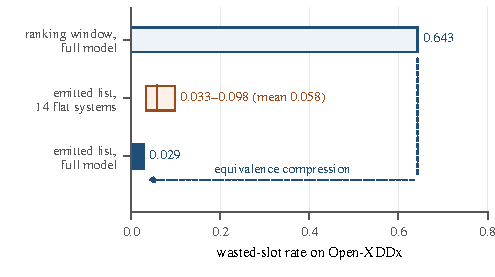
\includegraphics{figures/supp_redundancy.pdf}
\caption{Wasted-slot rate on Open-XDDx under one gold-blind lexical predicate, rendering one row of Table~\ref{tab:slots-mech} and the emitted-list column of Table~\ref{tab:slots-cross}. The ranking window that the case-specific organisation produces is an order of magnitude more redundant than any flat system's emitted list, because the organisation instantiates a concept once per competing family; after equivalence compression the emitted list of the full model falls below the least redundant flat system. The redundancy the compression stage removes is therefore created by the exploration this design performs and is not inherited from flat generation.}
\label{fig:redundancy}
\end{figure}
Compression is what converts wide multi-family exploration into a ranking whose slots are distinct, and the cost it pays is created by the exploration the same design chose to perform.
This also explains why removing both equivalence sites together is the only compression variant whose bound leaves the non-inferiority band in the main paper: the stage has more work to do in this architecture than a flat pipeline would ever give it.
The complementary half of the trade is that the flat systems buy their diversity by not exploring, and deliver the reference concept in $0.593$ of cases on average against $0.790$ for the full model (Section~\ref{sec:failvec}).

\section{State-Propagation Volume (extended analysis)}
\label{sec:propagation}

The main paper's factorial shows that withholding the evidence-conditioned score write-back costs accuracy, but it does not say how much revised state the write-back carries.
The deployed instrumentation counts, per case, the leaves whose score the local stage revised and the revisions the per-family cap discarded before write-back.
Table~\ref{tab:propagation} reports both against the size of the emitted ranking.

\begin{table}[tb]
\centering
\footnotesize
\setlength{\tabcolsep}{3pt}
\begin{tabular}{@{}lccccc@{}}
\toprule
Setting & Cap & Revised & Emitted & Ratio & Dropped \\
\midrule
Deployed            & $6$  & $22.9$ & $1.70$ & $13.5$ & $0$ \\
Write-back withheld & $6$  & $23.5$ & $1.66$ & $14.1$ & $0$ \\
Wider evidence      & $6$  & $23.7$ & $1.66$ & $14.3$ & $0$ \\
Cap of one          & $1$  & $23.0$ & $1.58$ & $14.5$ & $0$ \\
Cap removed         & none & $24.3$ & $1.62$ & $15.0$ & $0$ \\
\bottomrule
\end{tabular}
\caption{Revised local state per case on Open-XDDx. ``Revised'' counts leaves whose score the local stage rewrote, ``emitted'' the length of the final ranking, ``ratio'' their quotient, and ``dropped'' the revisions the per-family cap discarded at write-back. The counters exist only for this benchmark.}
\label{tab:propagation}
\end{table}

Three readings follow, and the first is a caveat rather than a result.
The counter records that revisions were computed, not that the decoder read them: it stands at $23.5$ per case in the configuration where the write-back is withheld, because the local stage still revises scores there and the switch governs only whether the global decoder sees them.
The quantity therefore sizes the state at stake and does not by itself contrast the two arms; the behavioural contrast is the factorial in the main paper.
Second, the state at stake is large relative to what is emitted: about $23$ revised scores per case against a ranking of $1.7$ entries, a ratio near $13.5$, so discarding the revisions is not a marginal perturbation of the decoder's input.
Third, the per-family cap is nearly inactive on this benchmark.
No configuration discarded a single revision at write-back, and moving the cap from one candidate per live family to unbounded changes the revised count only from $23.0$ to $24.3$, about one candidate in eighteen.
This is the mechanical explanation for the null result of the per-family cap ablation: the ablation varies a constraint that almost never binds, so the null is evidence about the operating point and not about the value of bounding decoding.

\section{Failure-Quality Vector (extended analysis)}
\label{sec:failvec}

Accuracy says how often a system is credited but not what kind of failure it commits, and two systems at the same score can be failing for reasons that call for different remedies.
For each system we partition the hundred DiagnosisArena cases into four exhaustive and mutually exclusive outcomes: credited at rank one; a delivery failure, where the reference concept binds to no emitted name even after the offline repair; an interface failure, where the unmodified interface credits nothing but the repair applied to the same emitted list credits rank one; and a ranking failure, where the concept is delivered and bindable yet not ranked first.
The partition keys off the scored decision rather than the rank column, because dense ranking lets several options tie at rank one without any of them being credited.
Table~\ref{tab:failvec} reports the vector.

\begin{table}[tb]
\centering
\footnotesize
\setlength{\tabcolsep}{2pt}
\begin{tabular}{@{}lccccc@{}}
\toprule
System & Credited & Delivered & Rank & Bind & Absent \\
\midrule
\textbf{APHHM}      & $\mathbf{0.71}$ & $0.79$ & $0.08$ & $\mathbf{0.02}$ & $\mathbf{0.19}$ \\
MEDDxAgent          & $0.62$ & $0.71$ & $0.09$ & $0.05$ & $0.24$ \\
MAC                 & $0.61$ & $0.67$ & $0.06$ & $0.04$ & $0.29$ \\
Dual-Inf            & $0.60$ & $0.70$ & $0.10$ & $0.02$ & $0.28$ \\
i-MedRAG            & $0.60$ & $0.67$ & $0.07$ & $0.03$ & $0.30$ \\
MDAgents            & $0.58$ & $0.67$ & $0.09$ & $0.04$ & $0.29$ \\
Self-refine         & $0.57$ & $0.62$ & $0.05$ & $0.08$ & $0.30$ \\
Flat rerank         & $0.56$ & $0.63$ & $0.07$ & $0.04$ & $0.33$ \\
CoT+RAG             & $0.55$ & $0.63$ & $0.08$ & $0.04$ & $0.33$ \\
Direct CoT          & $0.54$ & $0.61$ & $0.07$ & $0.05$ & $0.34$ \\
Chain-of-Diagnosis  & $0.54$ & $0.55$ & $0.01$ & $0.04$ & $0.41$ \\
Flat beam search    & $0.52$ & $0.60$ & $0.08$ & $0.03$ & $0.37$ \\
Self-consistent CoT & $0.52$ & $0.61$ & $0.09$ & $0.06$ & $0.33$ \\
Medprompt-style     & $0.52$ & $0.57$ & $0.05$ & $0.05$ & $0.38$ \\
Flat rerank (proxy) & $0.48$ & $0.59$ & $0.11$ & $0.05$ & $0.36$ \\
MedRAG              & $0.48$ & $0.52$ & $0.04$ & $0.05$ & $0.43$ \\
Flat rerank, ten    & $0.47$ & $0.59$ & $0.12$ & $0.03$ & $0.38$ \\
DiagnosisGPT-6B     & $0.14$ & $0.14$ & $0.00$ & $0.00$ & $0.86$ \\
\bottomrule
\end{tabular}
\caption{Failure-quality vector on DiagnosisArena Top-1. Columns are case fractions; ``rank'' is a ranking failure, ``bind'' an interface failure, ``absent'' a delivery failure, and these three sum to one with ``credited''. ``Delivered'' is the fraction whose reference concept binds to some emitted name under the unmodified interface. ``Flat rerank, ten'' is the ten-trajectory budget-matched control.}
\label{tab:failvec}
\end{table}

The full model holds the lowest delivery-failure fraction of the eighteen systems at $0.19$ against a range of $0.24$ to $0.86$, and the lowest interface fraction at $0.02$, matched only by one agent baseline.
Its advantage over the strongest baseline is therefore located: of the nine additional credited cases, delivery accounts for five and binding for three.
The vector is equally explicit about where the full model is not stronger.
Its residual error is more ranking-dominated than that of the baselines, with $0.276$ of the residual attributable to ranking against a flat mean of $0.155$, and eight cases are delivered and bindable yet not ranked first.
Delivery still dominates its residual at $0.655$, so the leading remaining loss is a concept never placed on the tree rather than one mishandled once there.
This is the intended shape for a staged system: the mechanisms remove the failures that are bookkeeping, and what remains is concentrated in the stage where additional evidence, rather than additional naming discipline, would help.
The locally backboned reference arm is the limiting case in the other direction, with $0.86$ delivery failures and no interface failures at all, consistent with the repair moving none of its cases in Section~\ref{sec:ial}.

\section{Coverage-Conditioned Conversion Is Not Cross-System Identifiable (extended analysis)}
\label{sec:conversion}

A natural summary of a staged system is its conversion rate, the share of delivered cases that are credited at rank one.
We computed it and report here why we do not use it as a comparison, since a reviewer computing it independently would reach a conclusion that the data do not support in either direction.

The full model converts $0.899$ of its delivered cases while delivering $0.790$; the flat systems convert between $0.797$ and $1.000$, mean $0.889$, while delivering $0.593$ on average.
Conversion and coverage are negatively correlated across the eighteen systems, with a Pearson correlation of $-0.540$, which is what a selection effect predicts: a system that delivers the reference concept less often conditions its conversion on a smaller and easier subset that its own behaviour selected.
Table~\ref{tab:conversion} shows that the comparison reverses completely when the conditioning set changes hands.

\begin{table}[tb]
\centering
\footnotesize
\setlength{\tabcolsep}{3pt}
\begin{tabular}{@{}lccccc@{}}
\toprule
System & $n_f$ & $c_f$ & $a_o(D_f)$ & $a_f(D_o)$ & $\Delta_o$ \\
\midrule
MEDDxAgent          & $71$ & $0.873$ & $0.775$ & $0.671$ & $+0.228$ \\
Dual-Inf            & $70$ & $0.857$ & $0.786$ & $0.671$ & $+0.228$ \\
MAC                 & $67$ & $0.910$ & $0.776$ & $0.671$ & $+0.228$ \\
i-MedRAG            & $67$ & $0.896$ & $0.791$ & $0.671$ & $+0.228$ \\
MDAgents            & $67$ & $0.866$ & $0.791$ & $0.646$ & $+0.253$ \\
Flat rerank         & $63$ & $0.889$ & $0.778$ & $0.633$ & $+0.266$ \\
CoT+RAG             & $63$ & $0.873$ & $0.762$ & $0.570$ & $+0.329$ \\
Self-refine         & $62$ & $0.919$ & $0.839$ & $0.658$ & $+0.241$ \\
Direct CoT          & $61$ & $0.885$ & $0.787$ & $0.608$ & $+0.291$ \\
Self-consistent CoT & $61$ & $0.852$ & $0.770$ & $0.595$ & $+0.304$ \\
Flat beam search    & $60$ & $0.867$ & $0.733$ & $0.570$ & $+0.329$ \\
Flat rerank (proxy) & $59$ & $0.814$ & $0.763$ & $0.532$ & $+0.367$ \\
Flat rerank, ten    & $59$ & $0.797$ & $0.780$ & $0.532$ & $+0.367$ \\
Medprompt-style     & $57$ & $0.912$ & $0.754$ & $0.582$ & $+0.316$ \\
Chain-of-Diagnosis  & $55$ & $0.982$ & $0.764$ & $0.582$ & $+0.316$ \\
MedRAG              & $52$ & $0.923$ & $0.731$ & $0.519$ & $+0.380$ \\
DiagnosisGPT-6B     & $14$ & $1.000$ & $0.571$ & $0.152$ & $+0.747$ \\
\bottomrule
\end{tabular}
\caption{Conversion under two directions of conditioning on DiagnosisArena. $D_f$ is the set of $n_f$ cases the flat system delivered and $c_f$ its conversion there, while $a_o(D_f)$ is the full model's credited rate on that same set. $D_o$ is the set of $79$ cases the full model delivered, on which its own conversion is $c_o = 0.899$; $a_f(D_o)$ is each baseline's credited rate there and $\Delta_o = c_o - a_f(D_o)$.}
\label{tab:conversion}
\end{table}

Conditioning on the flat system's delivered set, the full model's credited rate is lower for all seventeen baselines, with a mean difference of $-0.127$.
Conditioning on the full model's delivered set, the full model's conversion is higher for all seventeen, with a mean difference of $+0.319$.
Both directions are computed from the same records and the same scoring interface, and they disagree on every system.
The conditional quantity is thus determined by whose behaviour defined the conditioning set and does not identify a property of either system, so no ordering of systems can be read from it.
We accordingly treat the unconditional credited rate as the only endpoint invariant to this choice, which is what the main paper reports, and we retain the within-system utilisation figures of Section~\ref{sec:utilisation}, where the conditioning set is fixed while a single system's configuration varies.
Nothing in the main paper depends on a conversion comparison.

\section{Numerical Reconciliation of the Main-Paper Contrasts}
\label{sec:reconcile}

Every contrast in the main paper is reported at one of two calibres.
A marginal score is an average over the cases a configuration itself scored, and a paired difference is computed only over the cases both configurations scored.
The two calibres do not coincide whenever a configuration fails to emit a scorable ranking on some case, and a reader who mixes them will find pairs of published numbers that appear arithmetically incompatible.
This section publishes the underlying counts so that every figure in the main paper can be recomputed and the two calibres separated.

\subsection{Equivalence sites on MedCaseReasoning}

Table~\ref{tab:rec-eq-marg} gives both calibres for the four cells of the site design.
One configuration returned no scorable ranking on two cases, so the commonly scored sample is $98$ while three of the four cells were themselves scored on $100$.

\begin{table}[tb]
\centering
\footnotesize
\setlength{\tabcolsep}{4pt}
\begin{tabular}{@{}lcccc@{}}
\toprule
Configuration & $n$ own & Acc own & Correct/$98$ & Acc/$98$ \\
\midrule
Both sites on       & $100$ & $0.50$ & $50$ & $0.510$ \\
Build-time only     & $98$  & $0.50$ & $49$ & $0.500$ \\
Decision-time only  & $100$ & $0.50$ & $48$ & $0.490$ \\
Neither site        & $100$ & $0.42$ & $40$ & $0.408$ \\
\bottomrule
\end{tabular}
\caption{Accuracy at rank one for the equivalence-site design under both denominators. ``Own'' averages over the cases each configuration scored; the last two columns restrict all four cells to the $98$ commonly scored cases.}
\label{tab:rec-eq-marg}
\end{table}

The main paper's site table reports the own-denominator column, and the paired difference quoted in the same paragraph is computed on the $98$ commonly scored cases.
The apparent discrepancy between an eight-point marginal gap and a $10.2$-point paired difference is entirely this change of denominator: on the common sample the two cells stand at $50/98$ and $40/98$, and the ten cases separating them are all discordant in the same direction.

Table~\ref{tab:rec-eq-cell} gives the agreement table for every edge of the design.

\begin{table}[tb]
\centering
\footnotesize
\setlength{\tabcolsep}{2.5pt}
\begin{tabular}{@{}lccccr@{}}
\toprule
Contrast & Both & Ref.\ & Var.\ & Neither & $\Delta$ \\
\midrule
Both sites removed        & $40$ & $10$ & $0$ & $48$ & $+0.102$ \\
Build-time, routing absent & $40$ & $9$  & $0$ & $49$ & $+0.092$ \\
Routing, build-time absent & $38$ & $10$ & $2$ & $48$ & $+0.082$ \\
Build-time, routing kept   & $46$ & $4$  & $2$ & $46$ & $+0.020$ \\
Routing, build-time kept   & $49$ & $1$  & $0$ & $48$ & $+0.010$ \\
\bottomrule
\end{tabular}
\caption{Agreement tables for the equivalence-site edges on the $98$ commonly scored cases. ``Ref.'' counts cases the retained configuration alone gets right and ``Var.'' the removal variant alone; $\Delta$ is their difference over $98$. Exact conditional intervals are $[+0.039,+0.102]$, $[+0.030,+0.092]$, $[+0.004,+0.117]$, $[-0.034,+0.056]$ and $[-0.010,+0.010]$, with unadjusted $p$ of $0.002$, $0.004$, $0.039$, $0.688$ and $1.000$.}
\label{tab:rec-eq-cell}
\end{table}

The counts make one property explicit that the marginal table can only imply.
Removing either site alone costs $0.010$ and $0.020$, so the single-site marginals sum to $0.031$, while removing both costs $0.102$.
The joint removal is thus super-additive by $0.071$: the two sites are substitutable rather than additive, and the design retains its accuracy as long as equivalence is enforced somewhere, which is the mechanism claim the main paper makes and the reason a one-site ablation understates the stage.

\subsection{The reciprocal-rank column on DiagnosisArena}

The deployed system's credited ranks on DiagnosisArena are $71$ cases at rank one, $7$ at rank two, $1$ at rank three and $21$ uncredited.
The mean reciprocal rank over all credited depths is $0.7483$; truncating credit at depth two gives $0.7450$.
No baseline has a single case credited beyond rank two, so for all seventeen baselines the two definitions coincide and the reported values are unambiguous.
The column heading in the main paper's result table names depth two, while the value it carries for the deployed system is the untruncated mean, which exceeds the truncated value by $0.0033$ because of the one rank-three case.
The ordering of systems is unchanged under either definition, and the accuracy columns at depths one and two are unaffected.

\subsection{The two samples in the axis comparison}

The two axis contrasts respond differently to the change of sample, and Table~\ref{tab:rec-axis} separates them.

\begin{table}[tb]
\centering
\footnotesize
\setlength{\tabcolsep}{2.5pt}
\begin{tabular}{@{}llccccr@{}}
\toprule
Axis & Sample & $n$ & Both & Ref.\ & Var.\ & $\Delta$ \\
\midrule
Fixed ICD & all      & $100$ & $46$ & $25$ & $5$ & $+0.200$ \\
Fixed ICD & non-empty & $89$ & $46$ & $17$ & $5$ & $+0.135$ \\
Random    & all      & $100$ & $31$ & $40$ & $6$ & $+0.340$ \\
Random    & non-empty & $55$ & $31$ & $7$  & $6$ & $+0.018$ \\
\bottomrule
\end{tabular}
\caption{Axis contrasts against the case-adaptive reference under both samples. ``Non-empty'' restricts to cases on which the variant emitted a ranking at all. Exact intervals are $[+0.092,+0.266]$, $[+0.023,+0.209]$, $[+0.218,+0.415]$ and $[-0.118,+0.146]$, with unadjusted $p$ of $0.0003$, $0.017$, ${<}10^{-4}$ and $1.000$.}
\label{tab:rec-axis}
\end{table}

The fixed taxonomic axis remains behind the case-adaptive reference under both samples: the gap narrows from $0.200$ to $0.135$ when empty rankings are excluded and the interval stays clear of zero, which is the residual organizational effect the main paper reports.
The random axis behaves differently, its full-sample deficit of $0.340$ falling to $0.018$ with an interval spanning zero once the $45$ cases on which it emitted nothing are removed.

The two samples answer different questions, and the second does not correct the first.
Emitting no ranking at all is one of the ways a degenerate axis fails in the deployed pipeline, so the full-sample contrast is the effect of changing the axis on the system as it runs, which is the quantity the main paper reports.
Restricting to non-empty rankings conditions on a post-treatment variable and therefore does not estimate a causal contrast; it locates where an effect acts rather than rescaling it.
Read as a pair, the two rows say that a random organization damages the pipeline almost entirely by preventing the selector cascade from producing any evidence at all, whereas a fixed taxonomic organization also degrades the ranking that does get produced.
The same reasoning applies to the empty-ranking share in the axis cascade table (Table~\ref{tab:org-cascade}).

\subsection{Status of the equivalence band}

The main paper's bounds figure shades a symmetric five-point band and describes it as a pre-registered non-inferiority margin.
Two qualifications belong in the record.
The band is symmetric and therefore delimits an equivalence region rather than a one-sided non-inferiority margin.
Its width was fixed as a reporting convention before the compression variants were scored, but it was not lodged in an external registry, so it should be read as author-specified rather than as an independently auditable pre-registration.
Nothing in the analysis depends on the band: every variant in that figure is reported with its discordant counts and its exact interval, and a reader who prefers a different width can reapply it to the same counts.

\section{Paired Comparison Against Every Baseline}
\label{sec:paired-baselines}

The main result table reports unpaired accuracies.
Because all arms run on the same cases under the same interface, the paired comparison is available and is the more informative one, and Table~\ref{tab:rec-paired} gives it for the deployed system against each baseline on DiagnosisArena at rank one.

\begin{table}[tb]
\centering
\footnotesize
\setlength{\tabcolsep}{2.5pt}
\begin{tabular}{@{}lccccr@{}}
\toprule
Baseline & Acc & Ours & Theirs & $\Delta$ & $p_{\mathrm{Holm}}$ \\
\midrule
MEDDxAgent          & $0.62$ & $23$ & $14$ & $+0.09$ & $0.32$ \\
MAC                 & $0.61$ & $23$ & $13$ & $+0.10$ & $0.32$ \\
Dual-Inf            & $0.60$ & $24$ & $13$ & $+0.11$ & $0.32$ \\
i-MedRAG            & $0.60$ & $22$ & $11$ & $+0.11$ & $0.32$ \\
MDAgents            & $0.58$ & $26$ & $13$ & $+0.13$ & $0.27$ \\
Self-refine         & $0.57$ & $23$ & $9$  & $+0.14$ & $0.16$ \\
Flat rerank         & $0.56$ & $28$ & $13$ & $+0.15$ & $0.17$ \\
CoT+RAG             & $0.55$ & $30$ & $14$ & $+0.16$ & $0.16$ \\
Direct CoT          & $0.54$ & $28$ & $11$ & $+0.17$ & $0.10$ \\
Chain-of-Diagnosis  & $0.54$ & $30$ & $13$ & $+0.17$ & $0.12$ \\
Flat beam search    & $0.52$ & $31$ & $12$ & $+0.19$ & $0.07$ \\
Self-consistent CoT & $0.52$ & $30$ & $11$ & $+0.19$ & $0.06$ \\
Medprompt-style     & $0.52$ & $31$ & $12$ & $+0.19$ & $0.07$ \\
Flat rerank (proxy) & $0.48$ & $35$ & $12$ & $+0.23$ & $0.02$ \\
MedRAG              & $0.48$ & $35$ & $12$ & $+0.23$ & $0.02$ \\
Flat rerank, ten    & $0.47$ & $34$ & $10$ & $+0.24$ & $0.01$ \\
DiagnosisGPT-6B     & $0.14$ & $63$ & $6$  & $+0.57$ & ${<}0.001$ \\
\bottomrule
\end{tabular}
\caption{Paired comparison on DiagnosisArena at rank one, $n{=}100$ throughout, deployed system at $0.71$. ``Ours'' and ``Theirs'' count discordant cases in each direction; $\Delta$ is their difference over $100$; $p_{\mathrm{Holm}}$ is the exact conditional test adjusted across the seventeen comparisons.}
\label{tab:rec-paired}
\end{table}

The direction is positive against every arm and the discordance is asymmetric in every row.
Twelve of the seventeen differences clear $0.05$ unadjusted; four survive Holm adjustment across the family.
The four strongest baselines are not separated from the deployed system at this sample size: against the best of them the exact interval is $[-0.039,+0.204]$, which admits a small deficit.
We state this plainly because it bounds what the cross-benchmark table can support.
The claims the paper defends are mechanism claims, and they rest on the paired within-system contrasts of Sections~\ref{sec:reconcile} and \ref{sec:footprint}, where the same case set is scored under two configurations of one system and the discordant counts are large relative to the family.
The cross-system table establishes that the assembled system is competitive with the strongest published designs under a shared backbone and a shared corpus, and a separation claim against the leading agent baselines would require a larger sample than the fixed hundred-case subsets provide.

\section{Propagation Footprint of the Score Write-Back}
\label{sec:footprint}

Section~\ref{sec:propagation} sizes the state at stake but cannot contrast the two write-back configurations, because its counter records revisions computed rather than revisions read.
The behavioural complement is to compare the two configurations' emitted rankings case by case on Open-XDDx.
Of the hundred cases, $99$ emit a different set of labels when the write-back is withheld, $40$ change the label at the head of the ranking, and the mean overlap between the two emitted sets is $0.276$.
Withholding the write-back therefore does not perturb the decoder's output at the margin; it substitutes a largely different differential.

The scored consequence is selective rather than uniform.
On paired case-level micro-F1 the write-back improves $42$ cases, degrades $14$ and leaves $44$ unchanged, for a mean difference of $+0.073$ with a paired case-bootstrap interval of $[+0.035,+0.112]$ and an exact sign-test $p$ of $0.0002$.
Three of every four scored movements favour the write-back, and the fourteen degradations are the reason the effect is reported as a distribution rather than a uniform improvement.
Taken with Section~\ref{sec:propagation}, this gives the state-consistency invariant a behavioural reading: about $23$ revised scores per case reach a ranking of fewer than two emitted entries, the substitution is near-total in footprint, and its net effect on the benchmark endpoint is positive on three cases for every one it costs.

\section{Trajectory Diversity of the Budget-Matched Control}
\label{sec:diversity}

The budget-matched control draws ten trajectories through the flat pipeline and combines them by reciprocal-rank fusion, and it is the lowest-scoring shared-backbone arm on DiagnosisArena and sits in the lower third of the table on the other two.
An obvious objection is that the control wastes its budget on identical repetitions, which would make it a straw comparison rather than a matched one.
Table~\ref{tab:diversity} measures what the ten trajectories actually produce.

\begin{table}[tb]
\centering
\footnotesize
\setlength{\tabcolsep}{3pt}
\begin{tabular}{@{}lccccc@{}}
\toprule
Benchmark & Lists & Ident.\ & Heads & Jacc.\ & New \\
\midrule
DiagnosisArena   & $4.44$ & $0.07$ & $2.58$ & $0.547$ & $3.30$ \\
MedCaseReasoning & $4.13$ & $0.11$ & $2.48$ & $0.564$ & $3.23$ \\
Open-XDDx        & $7.95$ & $0.00$ & $2.21$ & $0.477$ & $8.92$ \\
\bottomrule
\end{tabular}
\caption{Per-case diversity of the ten trajectories. ``Lists'' is the number of distinct rankings among the ten, ``Ident.'' the fraction of cases on which all ten agree exactly, ``Heads'' the number of distinct first labels, ``Jacc.'' the mean pairwise Jaccard overlap of the candidate sets, and ``New'' the number of candidates the remaining nine trajectories add beyond the first.}
\label{tab:diversity}
\end{table}

The control is not degenerate.
On DiagnosisArena the ten trajectories produce $4.44$ distinct rankings per case, agree exactly on only seven cases in a hundred, nominate $2.58$ distinct first labels, and contribute $3.30$ candidates beyond those the first trajectory found; on Open-XDDx almost every trajectory is distinct and the ten jointly nominate nearly nine candidates the first pass missed.
The budget buys hypothesis diversity, and the fused ranking nonetheless scores $0.47$ on DiagnosisArena and delivers the reference concept in $0.59$ of cases against $0.79$ for the deployed system.
What the flat pipeline lacks is not candidates but a structure in which candidates compete: repetition proposes alternatives, and rank fusion counts them, but nothing in that loop decides between two nominations of the same concept or between two concepts under one differential.
This is the empirical content of the paper's position that the gain is attributable to organisation rather than to inference budget, and it is the reason the control is reported as a matched comparison rather than discarded.

\section{Retrieval Exposure Audit}
\label{sec:exposure}

All retrieval arms read one shared corpus, so a natural concern is that the corpus contains the benchmark material and that measured accuracy partly reflects retrieval of the answer.
We audit this offline in three layers, using the chunk identifiers each arm consumed and the corpus records those identifiers resolve to.

The first layer is provenance.
The MedCaseReasoning subset carries a source-article identifier for each of its hundred cases, and the corpus indexes carry $6013$ distinct article identifiers of the same kind.
The intersection is empty: no case in that subset originates from an article present in the corpus.
The DiagnosisArena and Open-XDDx subsets ship no provenance identifier, so this layer is undefined for them.

The second layer is textual.
For every case we take the union of the passages served to any retrieval arm and measure two quantities: whether a passage reproduces the case description, and whether a passage states the target diagnosis by name.
Reproduction of case text does not occur anywhere.
The largest eight-gram containment between a case vignette and any served passage is $0.026$ on MedCaseReasoning, $0.017$ on DiagnosisArena and $0.006$ on Open-XDDx, and no case on any benchmark exceeds $0.10$.
Naming of the target does occur, at rates that differ sharply by benchmark: some served passage states the target verbatim for $1$ case on DiagnosisArena, $16$ on MedCaseReasoning and $48$ on Open-XDDx.
The two findings should be read together.
A reference corpus that never names a disease would be useless for differential diagnosis, and the Open-XDDx rate is high because its targets are common conditions that any guideline collection discusses; contamination would be the reproduction of the benchmark instance, and that is what the containment measurement rules out.

The third layer asks whether the advantage depends on exposure.
Table~\ref{tab:exposure} restricts the comparison against the strongest MedCaseReasoning baseline to the cases whose target the corpus names and to those it does not.

\begin{table}[tb]
\centering
\footnotesize
\setlength{\tabcolsep}{4pt}
\begin{tabular}{@{}lcccc@{}}
\toprule
Stratum & $n$ & APHHM & Baseline & Margin \\
\midrule
Target named    & $16$ & $0.688$ & $0.438$ & $+0.250$ \\
Target not named & $84$ & $0.464$ & $0.202$ & $+0.262$ \\
\bottomrule
\end{tabular}
\caption{Accuracy on MedCaseReasoning stratified by whether any served passage names the target diagnosis. The baseline is the strongest arm on this benchmark.}
\label{tab:exposure}
\end{table}

Both systems score higher on the named stratum, which is expected since those cases are the ones the corpus covers.
The margin between them is $+0.250$ there and $+0.262$ on the unnamed stratum, a difference of $-0.012$ in the direction opposite to a contamination account.
Exposure raises the level for both systems and does not concentrate the advantage.
One caveat qualifies the audit: the deployed configuration did not persist per-case chunk identifiers, so exposure is measured from the retrieval baselines, which read the same index under the same passage budget, and is treated as a property of the case rather than of the system.

\section{Extended Analysis: Scope and Limitations}
\label{sec:extended-scope}

The analyses in Sections~\ref{sec:full-cohort}, \ref{sec:hazards}, \ref{sec:utilisation}, \ref{sec:interp}, \ref{sec:ial}, \ref{sec:decoupling}, \ref{sec:cases}, \ref{sec:slots}, \ref{sec:propagation}, \ref{sec:failvec}, \ref{sec:conversion}, \ref{sec:reconcile}, \ref{sec:paired-baselines}, \ref{sec:footprint}, \ref{sec:diversity}, and \ref{sec:exposure} recompute quantities from the persisted records of the evaluation passes already reported.
They introduce no additional inference and revise no claim in the main paper.
Three further measurements are new executions rather than recomputations: the second-judge re-scoring of the reasoning-recall endpoint, the live re-run of the leaf-injection diagnostic under the current judge contract, and the re-execution of the deployed Open-XDDx configuration that calibrates re-execution variability.
Each was carried out under the frozen protocol on the same case sets, and each corroborates the direction and the ordering of the corresponding result in the main paper; none of them revises a reported claim, and where a re-measured figure differs from the reported one, the difference is stated at the point of use.
Section~\ref{sec:reconcile} corrects two presentational defects in the main paper: a table of equivalence-site accuracies whose caption names the paired sample while its entries use each configuration's own denominator, and a reciprocal-rank column whose heading names depth two while one of its eighteen entries is untruncated.
Neither affects an ordering or a reported interval, and both are recomputable from the counts given there.
Thirteen limitations apply.
The stage assignment for the apparent-coverage bucket uses a lexical equivalence predicate, so separating parent absence from leaf absence within it still requires clinical adjudication.
The token axis is a reconstruction rather than a billed ledger, and the latency axis is uncontrolled for concurrency.
The interpretation endpoint remains a single-judge measurement, and although the reasoning-recall endpoint has since been re-scored by a second judge that preserves the ranking of every arm, the two judges differ in level by $-0.258$ on the full model and correlate at $0.404$ per case, so neither absolute level is validated against human scoring.
The reasoning-recall comparison also depends on what each arm persists: the evaluation projection reconstructs a reasoning trace from recorded fields, it recovers no rationale for one arm that does produce one, and that arm is therefore held out of the judge comparison rather than scored against an empty trace.
The cross-system redundancy panel uses a lexical predicate that agrees with the deployed predicate at $0.989$ on the endpoint where both are defined, but its agreement on flat emitted lists cannot be checked in the same way, and the one observed disagreement indicates that the deployed predicate can merge aetiologically distinct entities sharing a syndromic head.
The state-propagation counters exist only for Open-XDDx and record revisions computed rather than revisions read, so they size the state at stake without decomposing the write-back into the part that depends on which leaf receives which score and the part that follows from refreshing the shared state at all.
The re-execution measurement bounds how finely the state-consistency factorial can be read but does not itself supply that decomposition, and because it rests on a single repetition of one configuration it gives an order of magnitude for execution variability rather than a variance estimate.
The stage hazards are computed with a lexical matching predicate over structural records, so their terminal rates are lexical credit rates that differ from the judged endpoints, and only within-benchmark comparisons across transitions are meaningful.
The failure-quality partition inherits the coverage of the offline binding repair, so its interface column is a lower bound on interface-attributable failure and its delivery column is correspondingly an upper bound.
The paired cross-system comparison does not separate the deployed system from the four strongest baselines at a hundred cases, so the cross-system evidence supports competitiveness under a shared backbone rather than a ranking claim against those four.
The non-empty sample in the axis comparison conditions on a post-treatment variable, so the pair of calibres brackets the effect rather than estimating it.
The exposure audit measures the passages served to the retrieval baselines, because the deployed configuration did not persist per-case chunk identifiers, and its provenance layer is defined only on the one subset that ships source identifiers.
The propagation footprint compares emitted rankings and case-level scores between two configurations of one system on one benchmark, so it establishes that the write-back substitutes the differential rather than perturbing it, and does not replicate that finding across benchmarks.

\section{Statistical Evidence Map}

The contemporaneous contrast family contains the adaptive-axis, semantic-partition, evidence-conditioned score write-back, and selector comparisons, with Holm step-down used as conservative multiplicity control.
The axis comparison uses an exact paired binary test, the evidence-conditioned score write-back comparison uses a paired case-bootstrap that recomputes micro-F1, and the selector comparison serves as a negative control.
The semantic-partition comparison permutes equivalence-class membership under fixed cases; its responsive endpoints were selected through the admissibility audit.
The leaf-injection comparison appears separately as a retrospective diagnostic from the earlier judge configuration.

\begin{table*}[t]
\centering
\small
\begin{tabular}{@{}lllcc l@{}}
\toprule
Contrast & Endpoint & Effect & $p$ & $p_{\mathrm{Holm}}$ & Inference unit \\
\midrule
Adaptive vs.\ random axis pipeline & DA Top-1 & $+0.34$ & $3.1{\times}10^{-7}$ & $1.2{\times}10^{-6}$ & pipeline effect \\
Semantic vs.\ blind merge & MCR any-hit@5 & $+0.097$ & $0.015$ & $0.030$ & partition-level \\
Evidence-conditioned score write-back vs.\ none & OX micro-F1 & $+0.075$ & $4.0{\times}10^{-4}$ & $1.2{\times}10^{-3}$ & case-sampled \\
Case-relative vs.\ salience selector & DA Top-1 & $+0.04$ & $0.48$ & $0.48$ & negative control \\
\midrule
No injection vs.\ leaf injection & DA Top-1 & $+0.30$ & $1.5{\times}10^{-5}$ & --- & historical diagnostic \\
\bottomrule
\end{tabular}
\caption{Reported contrasts and their inferential units. Holm values control the four contemporaneous comparisons; leaf injection is listed as a retrospective diagnostic.}
\label{tab:confirmatory}
\end{table*}

\paragraph{Re-verification of the leaf-injection diagnostic (extended analysis).}
The leaf-injection contrast is listed separately in Table~\ref{tab:confirmatory} because its numbers were obtained under an earlier judge configuration and reused rather than re-measured.
We have since re-run the injected arm live under the judge contract that governs every other result reported here, holding the injection procedure, the case set, and the matching predicate fixed.
The uninjected reference is unchanged at Top-1 $0.72$; full-tree injection, which adds $16.1$ leaves per case, now yields Top-1 $0.40$ against the $0.42$ recorded in the retrospective pass, with reciprocal rank $0.608$.
The direction, the magnitude, and the conclusion drawn from the contrast are therefore not artefacts of the earlier configuration.
We keep the contrast listed separately because it was not part of the contemporaneous family and does not enter the multiplicity correction, but it no longer carries the additional caveat of being unverified under the current contract.

\paragraph{Coverage of the evidence.}
Table~\ref{tab:confirmatory} lists the contrasts that carry inferential weight; Figure~\ref{fig:evidence-map} states, for every kind of evidence in this paper, the benchmarks on which it exists.
The map separates two layers.
The descriptive and audit layer---the end-task comparison, the similar-call-count control, stage attribution, and ranking-window redundancy---is measured on all three benchmarks, so the claims resting on it are cross-benchmark claims.
The confirmatory layer is not: each mechanism contrast is measured on the single benchmark whose dominant failure stage it addresses, following the allocation described in Section~\ref{sec:full-cohort}.
We state the empty cells explicitly rather than leave them to be inferred, for two reasons.
They are the replication surface the main paper names as future work, and a mechanism evaluated on a benchmark where its target failure is rare would carry little information even if the arm were run, so the sparsity of the lower block reflects where the contrasts are informative and not only where computation was spent.

\begin{figure}[tb]
\centering
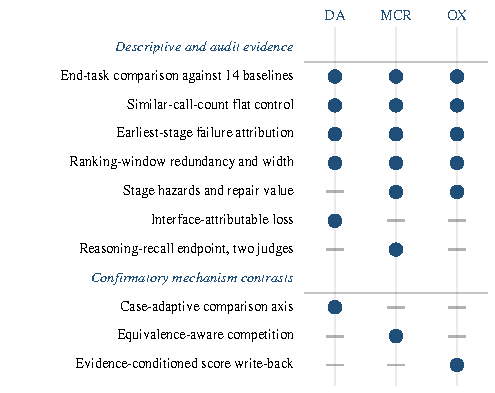
\includegraphics{figures/supp_evidence_map.pdf}
\caption{Coverage of the evidence reported in this paper and in the main paper. A filled marker indicates that the row is measured on that benchmark; a dash indicates that it is not evaluated. The descriptive and audit layer is complete or nearly complete across benchmarks, whereas each confirmatory mechanism contrast is measured on one benchmark, chosen as the one whose dominant failure stage that mechanism addresses (Figure~\ref{fig:funnel}).}
\label{fig:evidence-map}
\end{figure}

\section{Compression Variants and Structural Bounds}

This section reports variants of the equivalence-compression operator, including structurally invariant variants.
For binary Acc@1, paired binary intervals can be defined from endpoint-discordant cases on $n=98$ commonly scored MCR cases.
Each interval is the exact conditional interval on the discordant pairs, obtained by mapping a Clopper--Pearson interval for the proportion of discordant pairs favoring the full model back onto the difference scale; a paired difference cannot exceed the discordant count divided by $n$, so few moving cases imply a tight bound rather than low power.
Open-MRR@5 is summarized descriptively as a paired nonbinary endpoint.
The analysis plan used a $\pm5$ percentage-point non-inferiority margin for binary accuracy.
The main paper plots the same bounds against that margin; Table~\ref{tab:eq-equiv} adds the exact values and the number of cases whose delivered list changed.

The count-matched blind merge and its rank-1-size-matched variant are identities at @1 by construction and are evaluated with the responsive any-hit@5 and open-MRR@5 endpoints; the reported $p=0.015$ samples semantic partitions of the fixed cases.
Calibration-only routing is the one variant whose endpoint discordances run in both directions ($4$ favoring the full model and $2$ favoring the comparison).

\paragraph{Endpoint admissibility audit.}
For each candidate endpoint, we generated $200$ randomized equivalence re-partitions per case and counted cases whose endpoint changed.
Top-1 changed in $0/42$ audited MCR cases and $0/35$ audited DA cases, with null standard deviation exactly zero, as predicted for a deletion operator that retains each class's best-ranked member.
MCR any-hit@5 and open-MRR@5 were responsive and are therefore used for the semantic-compression analysis.
This audit distinguishes responsive endpoints from algebraic identities and defines the target endpoints for independent-subset confirmation.

\paragraph{Semantic structure beyond candidate count.}
Across the execution-site cross, the (candidates per case, accuracy) pairs are $(1.81,0.50)$, $(2.02,0.50)$, $(2.11,0.42)$, and $(4.64,0.50)$, showing that list length alone does not order accuracy.
The count-matched blind merge further preserves the deployed class-count and class-size profile while randomizing membership, yet is worse on both responsive endpoints.
The observed difference therefore tracks clinical equivalence structure beyond list shortening.

\paragraph{Partition-semantics randomization.}
The randomized control changes quotient structure while preserving the aggregate partition profile.
The synonym graph is complete in $0/35$ perturbable DA cases and $0/42$ perturbable MCR cases; $82.8\%$ and $85.1\%$ of draws, respectively, commit at least one quotient violation.
Across draws, the control wrongly merges an average of $1.99$ non-synonymous pairs and splits $1.98$ synonymous pairs.
It leaves $0.79$ synonymous duplicate pairs among surviving representatives, whereas the deployed single-linkage merge guarantees $0.00$.
The resulting permutation $p$-value quantifies sensitivity to class membership across randomized partitions of the fixed cases.

\paragraph{Closed-set binding audit.}
On DA, the compared compression configurations emit identical rank-1 labels in all $89$ gated cases, so the open-set Top-1 difference is exactly zero.
All $12$ option promotions under closed rematching already match the target under open scoring, and promotion is not selective for the target (Fisher $p=0.199$).
The $0.112$ closed-set increase is consequently localized to option binding, while the emitted disease concept remains unchanged.

\paragraph{Concept-identity predicate on DA.}
The concept-identity predicate scores $0.57$ option Top-1 on DA, compared with $0.71$ for the deployed configuration; unconditional synonym merging exceeds it by $0.11$ on the same caliber.
The concept-identity predicate yields more concept clusters than the deployed synonym-oriented predicate in $37$ cases and fewer in $0$.
The deployed advantage is concentrated in $10$ cases where a wider surface-form merge absorbs the target into the rank-1 representative class, which closed-set option rematching then credits.
This cross-caliber dissociation shows how closed-set option binding can reward a wider surface-form class even when clinical ranking is unchanged.

\paragraph{Why any-hit@5 is an identity for most variants.}
The full model delivers fewer than $k_{\mathrm{out}}{=}5$ candidates in $86$ of $98$ cases, so any-hit@5 usually reduces to whether the target is in the surviving set.
Because merging retains the best-ranked member of each class, matched labels remain represented, and seven of nine variants have zero moving cases on this endpoint.
Their identical values are structural identities.

\paragraph{Structural identities.}
Serial merge--calibration composition delivers the identical set, the identical rank-1 leaf, and zero moving cases on all three endpoints in this configuration; removing the family-level soft prior moves one case.
These configurations are therefore invariant or near-invariant on this evaluation subset.

\paragraph{Conditional effect sizes.}
Restricted to cases where the delivered list differs, the full model gains $+0.125$ Acc@1 over unconditional merge ($16$ cases) and $+0.107$ over frequency-matched random routing ($28$ cases).
These conditional estimates describe the changed-output cases alongside the full-sample intervals above.

\begin{table*}[t]
\centering
\small
\begin{tabular}{lccl}
\toprule
Variant & Changed outputs & Acc@1 $95\%$ CI & Structural status \\
\midrule
No decision-time routing & 94 & $[-1.4,+2.0]$ & open-MRR differs descriptively \\
Unconditional merge & 16 & $[-1.4,+2.0]$ & accuracy within margin \\
Calibration only & 82 & $[-2.5,+3.0]$ & bidirectional accuracy changes \\
Serial merge $\rightarrow$ calibrate & 7 & $[0,0]$ & endpoint identity \\
Frequency-matched random routing & 28 & $[-1.3,+3.1]$ & accuracy within margin \\
Count-matched blind merge & 33 & $[0,0]$ & rank-1 identity \\
Blind merge, rank-1 size matched & 26 & $[0,0]$ & rank-1 identity \\
Concept-identity predicate & 37 & $[-1.4,+2.0]$ & accuracy within margin \\
No family-level soft prior & 10 & $[-1.0,+1.0]$ & near-identity \\
\bottomrule
\end{tabular}
\caption{Compression variants against the full model, all of which vary \emph{which} policy performs the merge. ``Changed outputs'' counts cases with any delivered-list difference. The interval column reports paired binary Acc@1 bounds and is positive when the full model scores higher; open-MRR@5 is summarized descriptively. The complementary contrast that removes equivalence handling at both execution sites is reported in the main paper and is the only one to clear the $\pm5$ percentage-point margin.}
\label{tab:eq-equiv}
\end{table*}

\section{Axis Cascade and Organization Details}

Empty rankings uniformly reflect selector abstention with zero selected facts on the random axis, localizing them to the terminal state of the selector cascade (Table~\ref{tab:org-cascade}).

\begin{table}[tb]
\centering
\small
\begin{tabular}{@{}lcccc@{}}
\toprule
Axis & mean $n_{\mathrm{sel}}$ & $n_{\mathrm{sel}}{=}0$ & empty rank & @1 \\
\midrule
Case-adaptive & $4.94$ & $17$ & $1$ & $0.71$ \\
Fixed ICD & $0.65$ & $89$ & $11$ & $0.51$ \\
Random & $0.13$ & $97$ & $45$ & $0.37$ \\
\bottomrule
\end{tabular}
\caption{Selector cascade under three L1 axes on DA ($n{=}100$).}
\label{tab:org-cascade}
\end{table}

\section{State-Consistency Factorial Details}

Table~\ref{tab:state-detail} separates the family-cap variants from the decoder-only comparisons on the same score-updated tree.

\begin{table}[tb]
\centering
\small
\begin{tabular}{@{}p{2.35cm}ccc@{}}
\toprule
Variant & F1 & closed $-$ variant & $95\%$ CI \\
\midrule
Full model (closed) & $0.651$ & --- & --- \\
One candidate per family & $0.657$ & $-0.006$ & --- \\
Uncapped family frontier & $0.649$ & $+0.002$ & --- \\
Direct updated-score Top-$5$ & $0.593$ & $+0.058$ & $[0.028,0.085]$ \\
Updated-score-pool decoder & $0.610$ & $+0.041$ & $[0.013,0.069]$ \\
\bottomrule
\end{tabular}
\caption{OX cap and decoder variants at fixed budget with evidence-conditioned score write-back. Paired case-bootstrap intervals are reported for the decoder alternatives.}
\label{tab:state-detail}
\end{table}

\paragraph{Re-execution variability of the deployed configuration (extended analysis).}
Each entry in this factorial is a single execution of a pipeline that calls a language model at several stages, so a difference between two entries is interpretable only against the variation produced by executing the same configuration twice.
We measured that variation directly, by re-executing the deployed configuration from the persisted trees with no change of any kind and comparing the resulting leaf state against the deployed state case by case.
The re-execution is not a replay: the annotation stage regenerates part of the tree, the updated score changes on nearly every leaf that is written, and the recovered leaf posteriors agree exactly with the deployed ones on only $4$ of the $100$ cases.
Its end-task consequence is nevertheless small.
The re-executed deployed configuration scores micro-F1 $0.638$ against the $0.651$ obtained by the deployed run, a difference of $0.012$.

This measurement fixes the resolution at which the factorial can be read.
The contrast the main paper draws, between writing locally updated scores into the shared state and leaving that state unwritten, is $0.075$ with an interval whose lower end is $0.036$, so it is roughly six times the re-execution difference and its interval excludes differences of that size; it is not attributable to execution variability.
The cap variants, which sit within a percentage point or less of the full model, are of the same order as the re-execution difference and are therefore unresolved at this sample size rather than measured to be neutral, which is consistent with the main paper describing the cap as empirically secondary in this configuration.
One finer question this design cannot settle is how much of the write-back effect requires the specific correspondence between a leaf and its own updated score, as against the refresh of the shared state that any write also performs.
Separating the two calls for a deterministic replay of the annotation stage, which the non-determinism reported above precludes, together with a confirmation sample larger than a hundred cases; we leave the question open rather than settle it at the present resolution.

\section{Mechanistic Synthesis}

The audits converge on a single representation-centered account.
The case-adaptive axis creates families that support discriminative evidence selection; equivalence-aware competition converts string-level redundancy into concept-level frontier capacity; and evidence-conditioned score write-back carries local evidence into global arbitration.
Stage attribution then connects each observed error to the state transition or interface responsible for it.
Together, these mechanisms explain why APHHM preserves its end-task margins while using a smaller, semantically denser decision frontier.

\bibliography{references}

\end{document}